\section{RTE 及其解的结构简析}
\label{sec:preliminaries}

本节考察稳态辐射传输方程（RTE）解算子的基本性质，这些性质构成后续构建神经网络模型的理论基础。

首先，定义边界集合
\begin{equation}\label{eq:boundary}
    \Gamma_{\pm} := \{(\br,\bOmega) \mid \br\in\partial
    D,\;\bOmega\in\sS^{d-1},\;\mp\bn(\br)\cdot\bOmega<0 \},
\end{equation}
其中 $\bn(\br)$ 表示区域 $D$ 在边界点 $\br\in\partial D$ 处的外法向单位向量。辐射强度 $I(\br,\bOmega)$ 满足如下带有入射边界条件的 RTE：
\begin{equation}\label{eq:rte-with-bc}
    \begin{aligned}\bOmega \cdot \nabla I(\br,\bOmega) + \mut(\br) I(\br,\bOmega) & = \frac{\mus(\br)}{S_{d-1}} \int_{\sS^{d-1}} p(\bOmega,\bOmega^*) I(\br,\bOmega^*)\,\mathrm{d}{\bOmega^*}, &  & \text{在 } D\times\sS^{d-1}, \\
               I|_{\Gamma_{-}}(\br,\bOmega)                                   & = I_{-}(\br,\bOmega),                                                                                      &  & \text{在 }\Gamma_{-},
    \end{aligned}
\end{equation}
其中 $I_{-}$ 为 $\Gamma_{-}$ 上给定的入射强度函数，$S_{d-1} = \dfrac{2\pi^{d/2}}{\Gamma(d/2)}$ 为单位球面 $\sS^{d-1}$ 的表面积。

上述边值问题涉及的系数函数包括总截面 $\mu_t$、散射截面 $\mu_s$ 以及散射核 $p$。吸收截面定义为 $\mu_a = \mu_t - \mu_s$。散射核 $p(\bOmega,\bOmega^*)$ 描述了粒子从方向 $\bOmega^*$ 散射至方向 $\bOmega$ 的概率密度。我们假设散射核满足互易性（即 $p(\bOmega,\bOmega^*) = p(\bOmega^*,\bOmega)$）及归一化条件：
\begin{equation}
    \frac{1}{S_{d-1}}\int_{\sS^{d-1}} p(\bOmega,\bOmega^*) \,\mathrm{d}\bOmega^* = 1
    \quad\text{对几乎所有的 }\bOmega\in\sS^{d-1}.
\end{equation}
在许多应用场景中，通常还假设散射核具有旋转不变性，即 $p$ 仅依赖于散射角 $\theta = \arccos(\bOmega\cdot\bOmega^*)$。尽管本文提出的算法同样适用于一般散射核，为简化叙述，后文将基于该假设展开。

\subsection{解的存在唯一性与解算子}

本节回顾文献中关于解存在唯一性的相关结果。首先给出更一般情形下（即 $\mut$ 和 $\mus$ 同时依赖于 $\br$ 和 $\bm{v}$）在 $L^p$ 空间（$1\leq p\leq\infty$）中的存在唯一性定理。

\begin{theorem}[$L^p$ 空间中解的存在唯一性]\label{thm:existence-uniqueness-lp}
    假设：
    \begin{enumerate}
        \item 设 $\bm{v}=|\bm{v}|\bOmega\in V$，其中 $V\subset\mathbb{R}^3$ 为开集，$D\subset\mathbb{R}^d$ 为有界 Lipschitz 区域；
        \item $\mut:D\times V \to \mathbb{R}$ 非负，且 $\tau\mut\in L^\infty(D\times V)$。其中 $\tau(\br,\bm{v})$ 表示过点 $\br$ 沿方向 $\bm{v}$ 的射线在 $D$ 内的线段长度；
        \item $p: V\times V\to\mathbb{R}$ 非负且可测，并且
              \begin{equation}
                  \mua=\mut - \mus \geq 0.
              \end{equation}
    \end{enumerate}
    则对任意 $1\leq p \leq\infty$ 及允许的边界数据 $I_{-}$，辐射传输问题~\eqref{eq:rte-with-bc} 存在唯一解 $I$，并满足估计
    \begin{equation}
        \|\tau^{-\frac{1}{p}}I\|_{L^p(D\times V)} \leq e^{C_p}\|I_{-}\|_{L^p(\Gamma_{-};|\bn\cdot\bOmega|)}, \quad \text{其中 }
        C_p =\|\tau\mus\|_{L^\infty}.
    \end{equation}
    此外，若进一步假设 $\mut>0$，且存在某个 $\nu>0$ 使得
    \begin{equation}
        \frac{\mus}{\mut} \leq 1 - \nu,
    \end{equation}
    则有
    \begin{equation}
        \|\mut^{\frac{1}{p}}I\|_{L^p(D\times V)} \leq \nu^{-\frac{1}{p}}\|I_{-}\|_{L^p(\Gamma_{-};|\bn\cdot\bOmega|)},
    \end{equation}
    这一结果允许考虑 $\mut\to\infty$ 的极限情形，对渐近分析具有重要意义。
\end{theorem}

针对本文的具体设定及数值计算目标，我们主要采用下述定理，此时假设 $\mut$ 和 $\mus$ 仅依赖于空间位置 $\br$。在 $L^2(D\times\sS^{d-1})$ 空间中，存在唯一性表述如下。

\begin{theorem}[$L^2$ 空间中解的存在唯一性]\label{thm:existence-uniqueness-l2}
    假设区域 $D$ 有界，且 $\mua=\mut-\mus$、$\mus$ 与 $p$ 均为非负、有界、可测函数，即
    \begin{equation}
        \mua=\mut -\mus \geq 0, \quad \mus \geq 0, \quad \text{且} \quad \|\mua\|_{L^\infty(D)}<\infty, \|\mus\|_{L^\infty(D)}<\infty.
    \end{equation}
    并假设
    \begin{equation}
        \frac{1}{S_{d-1}}\int_{\sS^{d-1}}p(\bOmega,\bOmega^*)\,\mathrm{d}\bOmega^*=1, \quad\text{对几乎所有的 } \bOmega\in \sS^{d-1}.
    \end{equation}
    则对任意 $I_{-}\in L^2(\partial D\times\sS^{d-1})$，带边界条件的 RTE~\eqref{eq:rte-with-bc} 在 $L^2(D\times\sS^{d-1})$ 中存在唯一解 $I$。此外，存在常数 $C>0$，仅依赖于 $\text{diam}(D)$，$\|\mua\|_{L^\infty(D)}$ 和 $\|\mus\|_{L^\infty(D)}$，使得
    \begin{equation}
        \|\bOmega\cdot\nabla I\|_{L^2(D\times\sS^{d-1})}+\|I\|_{L^2(D\times\sS^{d-1})} \leq C \|I_{-}\|_{L^2(\partial D\times\sS^{d-1})},
    \end{equation}
\end{theorem}

在上述存在唯一性结果基础上，我们定义解算子
\begin{equation}
    \A: (I_{-};\mu_t,\mu_s,p) \mapsto I,
\end{equation}
即算子 $\A$ 将边界入射强度 $I_{-}$、总截面 $\mut$、散射截面 $\mus$ 以及散射核 $p$ 映射为计算域内的解 $I$。需要注意的是，算子 $\A$ 关于 $I_{-}$ 是线性的，而关于其他系数函数则一般是非线性的。

本文的目标是构造一种高效且精确的数值方法来近似解算子 $\mathcal{A}$。深入理解解算子的结构（即便仅是形式上的）对于设计高效且具有良好泛化能力的深度神经网络至关重要。为此，我们将 $\mathcal{A}$ 分解为若干计算上更易处理的子算子，从而为神经网络架构设计提供理论指导。

\subsection{解算子的结构分解}

为得到更便于分析与计算的解算子表示，我们将 RTE 改写为一个不动点方程。

定义 $\tau_{\br,\bOmega}(s_1,s_2)$ 为沿特征线从 $\br-s_1\bOmega$ 到 $\br-s_2\bOmega$ 的\emph{光学深度}：
\begin{equation} \label{eq:optical-depth}
    \tau_{\br,\bOmega}(s_1,s_2):=\int_{s_1}^{s_2} \mut(\br-s \bOmega) \,\mathrm{d}{s},
\end{equation}
并记 $s_{-}(\br,\bOmega)$ 为粒子沿方向 $\bOmega$ 从 $\br$ 逆向追溯至区域边界的距离：
\begin{equation}
    s_{-}(\br,\bOmega):= \inf \{s \geq 0 \mid \br-s\bOmega \in\partial D\}.
\end{equation}

首先考虑无散射的纯衰减问题：
\begin{equation}\label{eq:rte-sweep}
    \begin{aligned}\bOmega \cdot \nabla J_b(\br,\bOmega) + \mut(\br) J_b(\br,\bOmega) & = 0,                  &  & \text{在 } D\times\sS^{d-1}, \\
               J_b|_{\Gamma_{-}}(\br, \bOmega)                                    & = I_{-}(\br,\bOmega), &  & \text{在 }\Gamma_{-},
    \end{aligned}
\end{equation}
其解可表示为
\begin{equation}\label{eq:attenuation-op}
    J_b(\br, \bOmega)= \J I_{-}(\br, \bOmega) = e^{-\tau_{\br,\bOmega}(0,s_{-}(\br,\bOmega))} I_{-}\left(\br-s_{-}(\br, \bOmega)
    \bOmega, \bOmega\right).
\end{equation}
其中 $\J$ 称为衰减算子。

类似地，当源项 $I$ 已知时，方程
\begin{equation}\label{eq:lifting}
    (\bOmega\cdot\nabla + \mut)J = \mus I, \quad  J|_{\Gamma_{-}} = 0,
\end{equation}
的解为
\begin{equation}\label{eq:lifting-op}
    J=\cL I(\br, \bOmega) = \int_0^{s_{-}(\br, \bOmega)} e^{-\tau_{\br,\bOmega}(0,s)}\mus(\br-s\bOmega)I(\br-s\bOmega, \bOmega)\,\mathrm{d}{s},
\end{equation}
其中 $\cL$ 称为提升算子（Lifting Operator）。此外，定义散射算子
\begin{equation}\label{eq:scattering-op}
    \cS I(\br, \bOmega) = \frac{1}{S_{d-1}}\int_{\sS^{d-1}} p(\bOmega, \bOmega^*)I(\br, \bOmega^*) \,\mathrm{d}{\bOmega^*}.
\end{equation}

通过对算子 $\bOmega \cdot \nabla + \mut(\br)$ 求逆，RTE 边值问题可改写为积分形式的算子方程
\begin{equation}\label{eq:rte-op-form}
    I = \cL\cS I + \J I_{-},
\end{equation}
即一个第二类 Fredholm 积分方程，其中 $\cL\cS I$ 表示散射贡献，$\J I_{-}$ 表示边界条件贡献。

该方程可通过不动点迭代求解：
\begin{equation}\label{eq:fixed-point-iteration}
    I^{m+1} = \cL\cS I^m + \J I_{-}.
\end{equation}
当初始猜测取为 $I^0 = \J I_{-}$ 时，该迭代与经典的源迭代方法
~\cite{adams2002fast}形式一致。进一步地，根据~\cite{egger2014lp} 的结论，我们有如下定理：
\begin{theorem}[谱半径估计]\label{thm:spectral-radius}
    在定理~\ref{thm:existence-uniqueness-lp} 的假设条件下，对任意 $1\leq p\leq \infty$，不动点算子 $\cL\cS$ 的谱半径满足
    \begin{equation}
        \rho_p(\cL\cS) := \lim_{n\to\infty}\sqrt[n]{\| (\cL\cS)^n \|_{L^p(D\times V;\tau^{-1})}} \leq 1 - e^{-C_p} < 1.
    \end{equation}
    这表明谱半径被一致地界定在 1 之下，从而保证迭代收敛到 RTE 的唯一解。
\end{theorem}因此，解算子可展开为级数形式：
\begin{equation}\label{eq:soln-op-series}
    \A[\mu_t,\mu_s,p] I_{-} = \sum_{n=0}^\infty(\cL\cS)^n\J I_{-}.
\end{equation}
这一迭代结构为神经网络架构设计提供了重要启发，我们可以设计一个深度网络的框架自然地对应这一迭代过程。

在传统文献中，散射截面 $\mus$ 往往被并入散射算子 $\mathcal{S}$，而不是包含在提升算子 $\mathcal{L}$ 中。
但是在本文中，提升算子 $\mathcal{L}$ 负责刻画沿特征线的传输性质，$\mathcal{S}$ 主要处理角度耦合。因此为了适配本文所提出模型的特定结构，我们将 $\mus$ 放置于 $\mathcal{L}$ 中。这样的划分既便于在框架中有效整合 $\mus$，又保持了与网络结构设计之间的协调一致。

\subsection{格林函数与解算子}

本小节从分布核的角度考察解算子 $\A$，旨在应用格林函数理论来进一步理解 RTE 的解算子结构，给后续的深度学习模型设计提供理论基础。

设 $G(\br,\bOmega,\br',\bOmega')$ 为如下方程（在分布意义下）的解：
\begin{equation}\label{eq:rte-greens-function}
    \begin{aligned}
        (\bOmega \cdot \nabla + \mu_t)G & =  \mus\cS G, \quad                                     &  & \text{在 } D\times\sS^{d-1}, \\
        G|_{\Gamma_{-}}                 & = \delta_{\{\br'\}}(\br)\delta(\bOmega-\bOmega'), \quad &  & \text{在 }\Gamma_{-},
    \end{aligned}
\end{equation}
其中 $(\br',\bOmega')\in\Gamma_{-}$ 为参数；$\delta_{\{\br'\}}$ 和 $\delta(\bOmega)$ 分别表示边界上的 Dirac 分布和角度空间中的 Dirac $\delta$ 函数。$G$ 称为 RTE 的格林函数，表示系统对边界点源的响应。

由于解算子相对于边界条件具有线性性，因此由格林函数理论可知，RTE 的解 $I$ 可表示为如下积分形式：
\begin{equation} \label{eq:rte-op}
    I(\br,\bOmega) = \int_{\Gamma_{-}}
    G(\br,\bOmega,\br',\bOmega')I_{-}(\br',\bOmega')\,\mathrm{d}{\br'}\,\mathrm{d}{\bOmega'}
    = \A[\mu_t,\mu_s,p] I_{-}(\br,\bOmega).
\end{equation}

上述公式表明，若能确定所有边界点 $(\br',\bOmega')$ 的格林函数 $G(\br,\bOmega,\br',\bOmega')$，那最后的解就可通过积分算子直接获得。接下来的重点即为如何获取格林函数 $G$。

把上一个章节中的不动点迭代和级数展开引入，可通过如下迭代表示格林函数 $G$ ：
\begin{equation}\label{eq:greens-function-iterations}
    \begin{aligned}
         & G^{m+1} =\cL\cS G^m+G^0= \cL\cS G^m+\J\left(\delta_{\{\br'\}}(\br)\delta(\bOmega-\bOmega')\right).
    \end{aligned}
\end{equation}
或表示为级数展开：
\begin{equation}\label{eq:greens-function-series}
    G(\br,\bOmega,\br',\bOmega') = \sum_{n=0}^\infty(\cL\cS)^n\J
    \left(\delta_{\{\br'\}}(\br)\delta(\bOmega-\bOmega')\right).
\end{equation}
进而解算子的结构可以表示为：
\begin{equation} \label{eq:rte-op1}
    \begin{aligned}
        \A[\mu_t,\mu_s,p] I_{-}(\br,\bOmega) & = \int_{\Gamma_{-}}
        G(\br,\bOmega,\br',\bOmega')I_{-}(\br',\bOmega')\,\mathrm{d}{\br'}\,\mathrm{d}{\bOmega'} \\
                                             & = \sum_{n=0}^\infty\int_{\Gamma_{-}}(\cL\cS)^n \J
        \left(\delta_{\{\br'\}}(\br)\delta(\bOmega-\bOmega')\right)I_{-}(\br',\bOmega')\,\mathrm{d}{\br'}\,\mathrm{d}{\bOmega'}.
    \end{aligned}
\end{equation}

若 $\mut$, $\mus$ 和 $p$ 给定且固定，一个朴素的想法是使用多层感知机（MLP）直接拟合格林函数 $G(\mathbf{r}, \Omega, \mathbf{r}', \Omega')$。然而，$\mu_t$ 和 $\mu_s$ 是空间依赖函数，甚至可能是不连续的，而 $p(\Omega, \Omega^\ast)$ 定义在 $\mathbb{S}^{d-1} \times \mathbb{S}^{d-1}$ 上。格林函数对这些参数函数的依赖关系可能极其复杂。在最后的实验章节里面，我们将展示这种朴素设计在泛化能力方面的劣势。因此，为了训练一个适用于复杂 $\mu_t$, $\mu_s$ 和 $p$ 的解算子，必须在神经算子的结构设计中充分考虑解对参数函数的特定依赖方式。

\section{网络结构}
\label{sec:network-architecture}

我们的目标是学习 RTE 定义在固定的有界区域 $D$ 上的解算子：
\begin{equation}\label{eq:solution-op}
    \ANN \approx \A: (I_{-}; \mut, \mus, p) \rightarrow I.
\end{equation}
为简明起见，后续讨论中省略对 $D$ 的显式记号。

具体而言，解算子 $\ANN$ 由其分布核（即~\eqref{eq:rte-op} 中的格林函数）给出的积分表示
\begin{equation}\label{eq:greens-integral-nn}
    I(\br, \bOmega)\approx I^\text{NN}(\br,\bOmega) = \ANN[\mut,\mus,p] I_{-} = \int_{\Gamma_-} G^{\text{NN}}(\br, \bOmega, \br', \bOmega') I_{-}(\br', \bOmega') \diff{\br'} \diff{\bOmega'},
\end{equation}
其中 $G^{\text{NN}}$ 是由深度神经网络参数化的格林函数。
\begin{figure}[!htp]
    \centering
    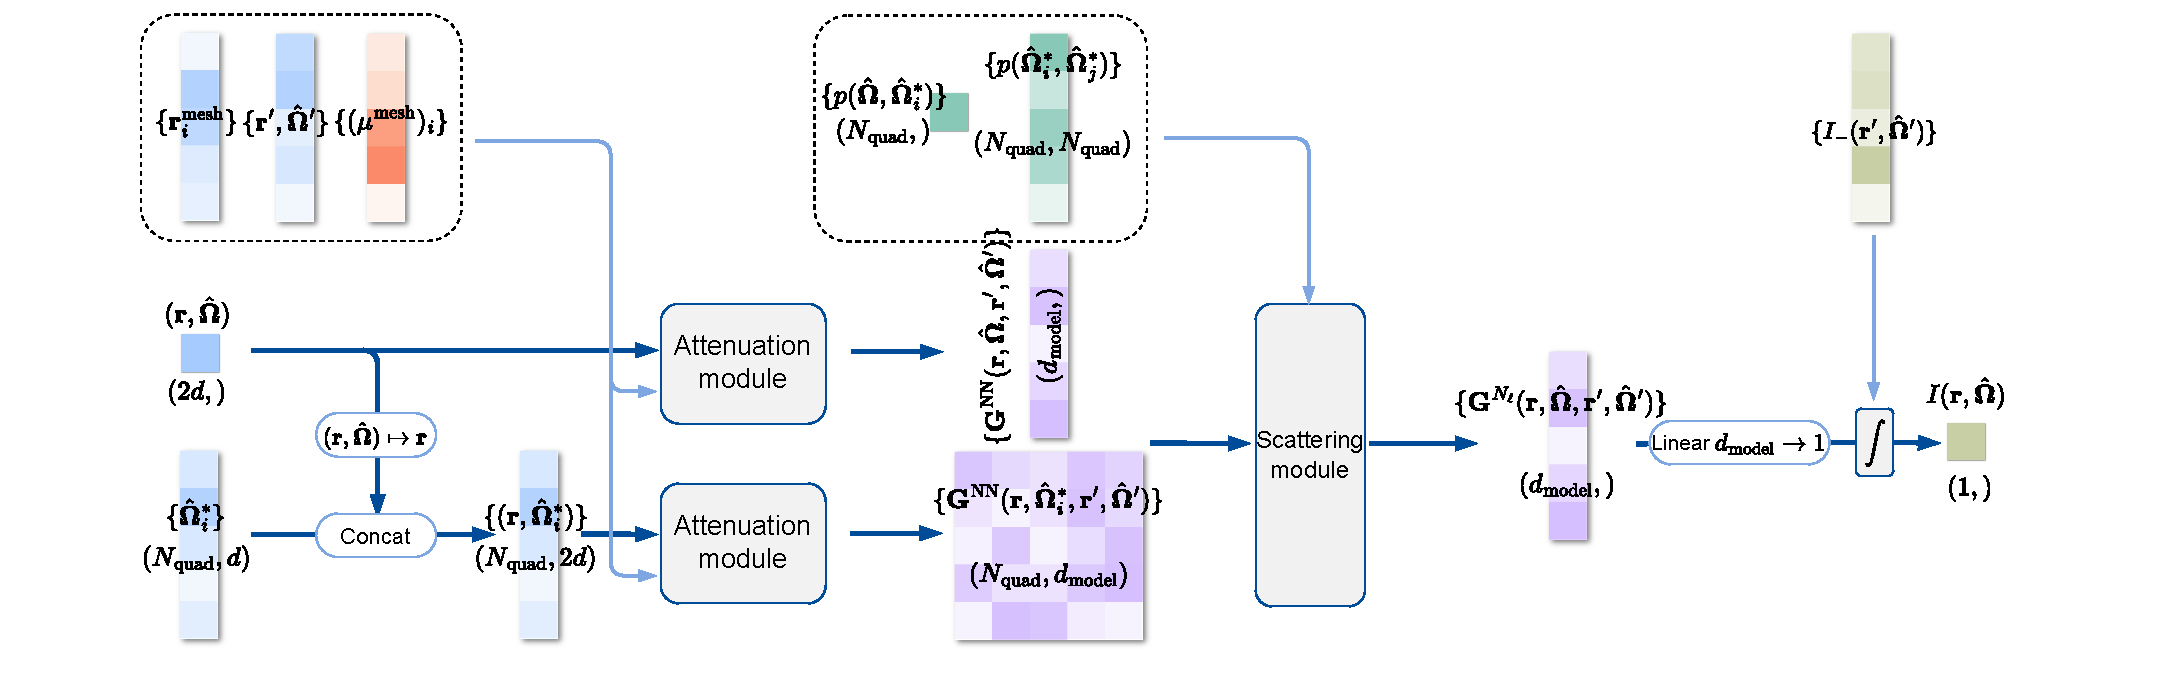
\includegraphics[width=1\textwidth]{figures/architecture.pdf}
    \bicaption{DeepRTE 网络架构。}{DeepRTE network architecture. }\label{fig:arch-overview}
\end{figure}
DeepRTE 的整体结构如图~\ref{fig:arch-overview} 所示，由受~\eqref{eq:greens-function-iterations} 中迭代过程启发的若干模块组成，并在有限步内进行迭代。该图展示了各种输入在整个过程中的变化。衰减模块处理相空间坐标和系数以近似算子 $\J$ 和 $\cL$，随后散射模块处理角度求积计算，同时进行算子迭代。最终，格林函数 $G^{\text{NN}}$ 与边界条件相乘并在 $\Gamma_-$ 上积分来计算辐射强度。

输入特征包括：
\begin{itemize}\label{list:attenuation-inputs}
    \item $(\br,\bOmega)$：待评估解的相空间坐标；
    \item $(\br',\bOmega')$：边界$\Gamma_-$ 的相空间坐标，在~\eqref{eq:greens-integral-nn} 中的边界积分中被使用；
    \item $\{{(\mu_t^{\text{mesh}})}_i=\mu_t(\br^{\text{mesh}}_i)\}$，$\{{(\mu_s^{\text{mesh}})}_i=\mu_s(\br^{\text{mesh}}_i)\}$，$\{\br^{\text{mesh}}_i\}$：总截面系数和散射截面系数在空间网格点上的取值，以及对应的空间网格点坐标。网格既可以是均匀的，也可以是结构化或非结构化的稀疏网格。
\end{itemize}
这些特征会被输入衰减模块，该模块显式建模了解算子对函数 $\mut$ 和 $\mus$ 的依赖。
衰减模块的输出随后与以下特征结合：
\begin{itemize}
    \item  $\{p(\bOmega, \bOmega^*_i)\}$，$\{\omega_i\}$：在任意角度 $\bOmega$、求积点 $\bOmega^*_i$ 上的相函数 $p$，以及对应的求积权重 $\omega_i$；
    \item  $\{p(\bOmega^*_i, \bOmega^*_j)\}$，$\{\omega_j\}$：在求积点 $(\bOmega^*_i, \bOmega^*_j)$ 上的相函数 $p$，会在网络中残差连接及多步散射更新的计算中被使用。
\end{itemize}
以上信息被输入散射模块，该模块用于模拟迭代过程 \eqref{eq:fixed-point-iteration}。
最后，散射模块的输出通过一个线性层投影为标量格林函数 $G^{\text{NN}}$。将 $G^{\text{NN}}$ 与边界条件 $I_{-}(\br',\bOmega')$ 相乘，并在边界相空间坐标 $(\br',\bOmega')$ 上积分，即可得到任意相空间点 $(\br,\bOmega)$ 上的解 $I$。

作为总结，我们在算法~\ref{alg:green-function} 中概括给出了从输入到格林函数的计算流程。关键思想和组成模块的细节将在后续小节中依次说明。

\begin{algorithm}[htp!]
    \caption{格林函数}\label{alg:green-function}
    \SetAlgoLined
    \KwIn{$\br,\bOmega,\br^{\prime},\bOmega^{\prime},\{\br_i^{\text{mesh}}\}, \{{(\mut^{\text{mesh}})}_i\},\{{(\mus^{\text{mesh}})}_i\},\{p(\bOmega,\bOmega^*_i)\},\{p(\bOmega^*_i,\bOmega^*_j)\}, \{\omega_j\}$}
    \KwOut{$g$}

    \BlankLine

    \emph{计算衰减模块的输出$\bm{g}\in \mathbb{R}^{d_{\text{model}}}$}\;
    $\bm{g}=\hyperref[alg:attenuation-module]{\text{AttenuationModule}}(\br,\bOmega,\br^{\prime},\bOmega^{\prime},\{\br_i^{\text{mesh}}\},\{{(\mut^{\text{mesh}})}_i\},\{{(\mus^{\text{mesh}})}_i\})$\;

    \emph{计算角度求积点处的衰减模块输出$\bm{g}^*_j\in \mathbb{R}^{d_{\text{model}}}$}\;
    $\{\bm{g}^*_j\}=\hyperref[alg:attenuation-module]{\text{AttenuationModule}}(\br,\{\bOmega_j^*\},\br^{\prime},\bOmega^{\prime},\{\br_i^{\mathrm{mesh}}\},\{{(\mut^{\mathrm{mesh}})}_i\}, \{{(\mus^{\mathrm{mesh}})}_i\})$\;

    \emph{调用散射模块模拟迭代更新$\bm{g}\in \mathbb{R}^{d_{\text{model}}}$}\;
    $\bm{g}\gets\hyperref[alg:scattering-module]{\text{ScatteringModule}}(\bm{g}, \{\bm{g}^*_j\}, \{p(\bOmega,\bOmega^*_i)\},\{p(\bOmega^*_i,\bOmega^*_j)\}, \{\omega_j\})$\;

    \emph{将潜在特征向量投影至标量格林函数$g\in\mathbb{R}$}\;
    $g = \text{LinearNoBias}(\bm{g})$\;

    \Return{$g$}\;
\end{algorithm}


\subsection{衰减模块}\label{sec:attenuation-module}

衰减模块利用神经网络给出算子 $\J$ 和 $\cL$ 的格林函数离散表示。二者可统一写成
\begin{equation}\label{eq:L-op}
    \int_0^{s_{-}(\br, \bOmega)} e^{-\tau_{\br,\bOmega}(0,s)}u(\br-s\bOmega, \bOmega)\diff{s},
\end{equation}
其中，对 $\cL$ 有 $u(\br, \bOmega)=\mus(\br)I(\br, \bOmega)$；对 $\J$ 则有 $u(\br, \bOmega)=I_-(\br-s_-\bOmega, \bOmega)\delta_{\{s\}}(s_-)$。这表明，获得沿特征线 $\br-s \bOmega$ 的格林函数表示至关重要。

在本文中，沿特征线的辐射场由维度为 $d_{\text{model}}$ 的离散向量表示：
\begin{equation}
    \bG^{\text{NN}} =
    \begin{pmatrix}
        G(\br-s_1 \bOmega, \bOmega; \br', \bOmega') \\
        \vdots                                      \\
        G(\br-s_{d_{\text{model}}} \bOmega, \bOmega; \br', \bOmega')
    \end{pmatrix}\in \mathbb{R}^{d_{\text{model}}}.
\end{equation}
参数 $d_{\text{model}}$ 表示离散表示的维度，可理解为沿特征线的采样点数量。每个分量 $G(\br-s_i \bOmega, \bOmega; \br', \bOmega')$（其中 $s_i\in (0,s_-(\br,\bOmega))$）对应特征线上某一点处格林函数的取值。需要强调的是，$s_i$ 的具体位置并未在网络结构中显式出现。

如此得到的表示既能捕捉主要的衰减特性，又通过低维潜在向量保持了计算的可控性。

神经网络输出 $\bG^{\text{NN}}$ 依赖于相空间坐标 $(\br,\bOmega)$ 与 $(\br',\bOmega')$ 以及系数 $\mut$。在实现上，我们采用如下神经网络结构：
\begin{equation}\label{G_equation}
    \bG^{\text{NN}}(\br,\bOmega,\br^{\prime},\bOmega^{\prime}; \mut) =\text{MLP}\left(\br,\bOmega,\br^{\prime},\bOmega^{\prime},\tau_-^{\text{NN}}\right),
\end{equation}
其中光学深度 $\tau_-^{\text{NN}}$ 由名为 OpticalDepthNet 的专用子网络计算。OpticalDepthNet 学习总截面 $\mut$ 决定光学深度的复杂方式，从而刻画 $\mu_t$ 对格林函数的影响。
随后，多层感知机（MLP）在此基础上融合空间与角度信息，输出沿特征线的截断格林函数表示。

衰减模块的整体结构见图~\ref{fig:attenuation-module}，该图展示了网络将空间坐标 ($\br,\br'$)、角度变量 ($\bOmega,\bOmega'$) 和截面 ($\mut,\mus$) 作为输入。OpticalDepthNet 子模块首先计算沿特征线的光学深度 $\tau_-^{\text{NN}}$。然后，这些特征由 MLP 处理，生成截断的格林函数表示 $\bG^{\text{NN}}\in\mathbb{R}^{d_{\text{model}}}$，该表示在离散点 $\br-s_i\bOmega$（特征线上的圆圈）处对辐射场进行采样。该架构有效地捕捉了局部散射效应和非局部衰减，同时通过降维保持了计算的可处理性。

更多算法细节可以参考算法~\ref{alg:attenuation-module}。光学深度网络 $\tau_-^{\text{NN}}$（OpticalDepthNet）的细节将在下一小节中给出。

\begin{figure}
    \centering
    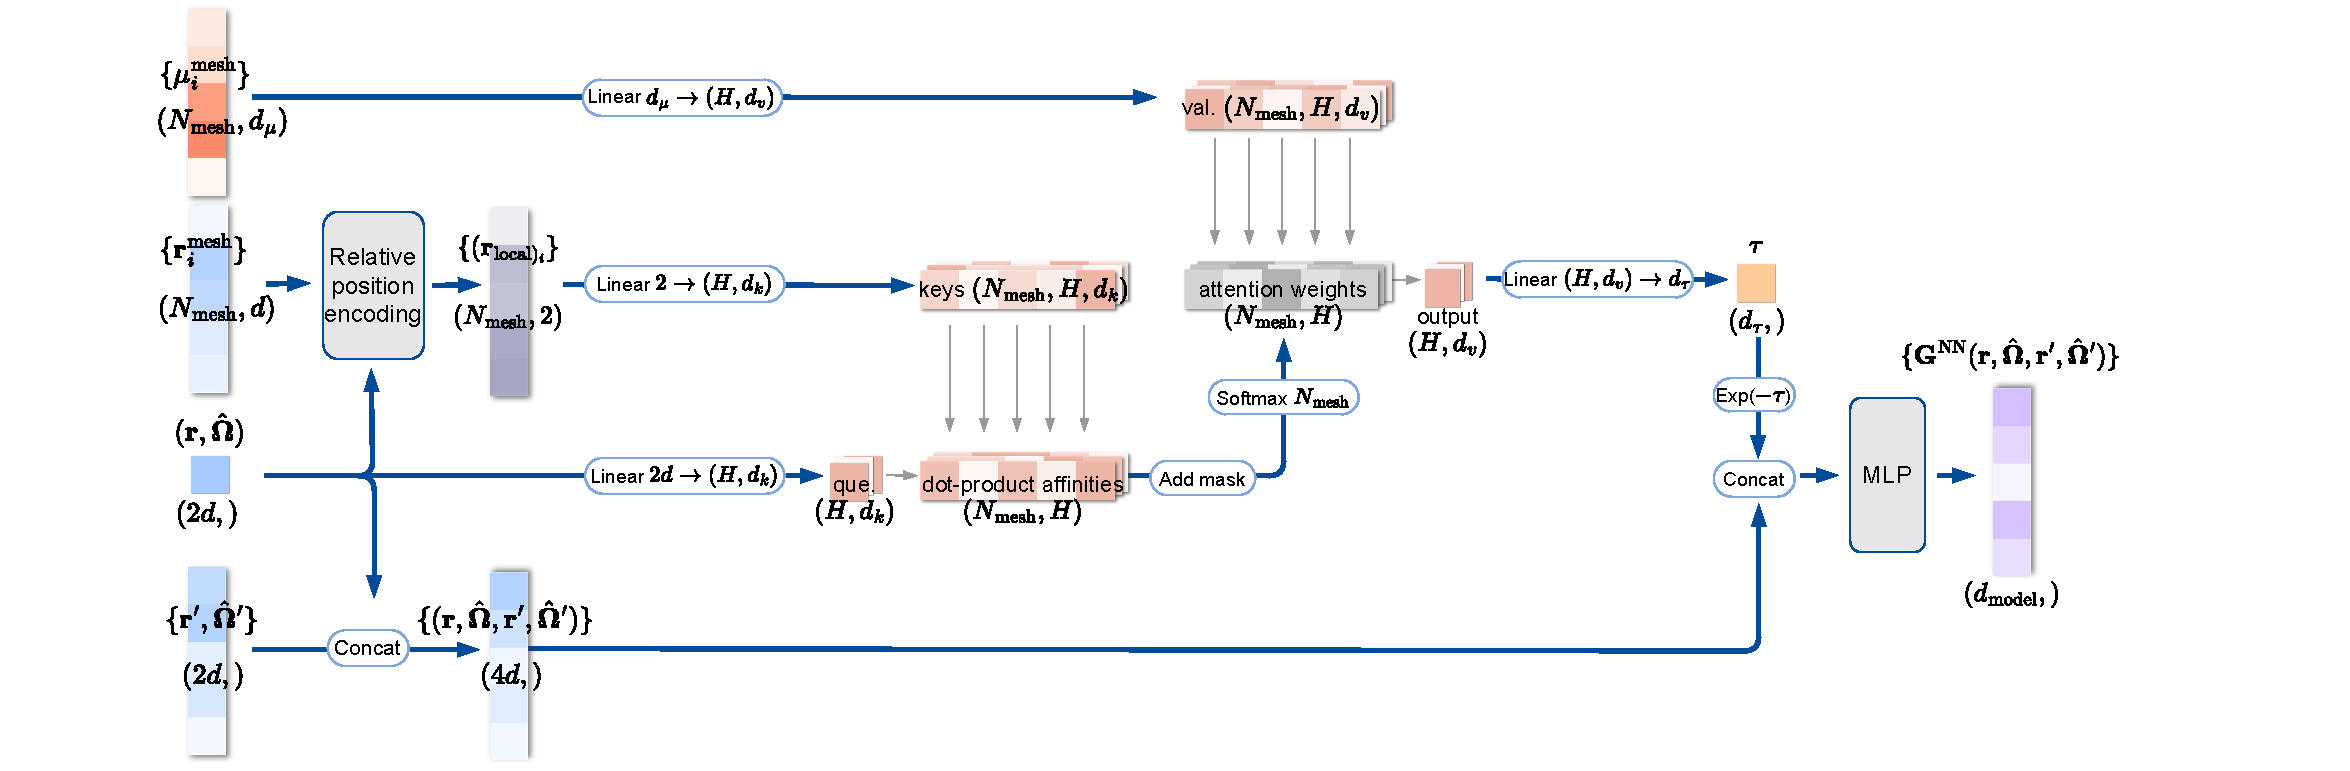
\includegraphics[width=1\textwidth]{figures/attenuation_module.pdf}
    \bicaption{
        DeepRTE衰减模块架构。
    }{Attenuation module architecture.}\label{fig:attenuation-module}
\end{figure}
\begin{algorithm}[htp!]
    \caption{衰减模块（Attenuation Module）}\label{alg:attenuation-module}
    \SetAlgoLined
    \KwIn{$\br,\bOmega,\br^{\prime},\bOmega^{\prime},\{\br_i^{\text{mesh}}\},\{{(\mut^{\text{mesh}})}_i\},\{{(\mus^{\text{mesh}})}_i\}, N_{\text{mlp}}=4,d_{\text{mlp}}=128,d_{\text{model}}=16$}
    \KwOut{$\bm{g}$}

    \BlankLine

    \emph{利用光学深度网络计算特征}\;
    $\tau_{-}^{\text{NN}} = \hyperref[alg:optical-depth-net]{\text{OpticalDepthNet}}(\br,\bOmega,\{\br_i^{\text{mesh}}\},\{{(\mut^{\text{mesh}})}_i\},\{{(\mus^{\text{mesh}})}_i\}, d_k=12, H=2)$\;
    $\bm{z} = \text{concat}(\br, \bOmega, \br^{\prime}, \bOmega^{\prime}, e^{-\tau_{-}^{\text{NN}}})$\;

    \emph{通过多层感知机处理特征, $\bm{z} \in \mathbb{R}^{d_{\text{mlp}}}$}\;
    \For{$l\in[1,\ldots,N_{\text{mlp}-1}]$}{
        $\bm{z}\gets\text{tanh}(\text{Linear}(\bm{z}))$\;
    }

    \emph{将特征投影到输出空间, $\bm{g} \in \mathbb{R}^{d_{\text{model}}}$}\;
    $\bm{g} = \text{Linear}(\bm{z})$\;

    \Return{$\bm{g}$}\;
\end{algorithm}

\subsubsection{光学深度网络}
光学深度网络用于刻画沿特征线的累积影响。传统的沿特征线数值积分方法往往面临较大计算代价。例如，由 \eqref{eq:optical-depth} 可知，若要在每个相空间点上计算下述光学深度
\begin{equation}
    \tau_{-,t}(\br,\bOmega):=\tau(0, s_-(\br, \bOmega))=\int^{s_-(\br, \bOmega)}_{0} \mut(\br-s\bOmega) \diff{s},
\end{equation}
对每个 $(\br,\bOmega)$ 显式进行特征线积分都十分耗时，对高度复杂的几何形状甚至难以实施，同时在辐射输运问题中还需要快速的计算方法。所以我们需要使用一种高效的近似方法来计算 $\tau_{-,t}(\br,\bOmega)$，而传统的数值方法往往难以满足这一需求。

于是我们设计了一个专门的神经网络子模块 OpticalDepthNet 来高效近似光学深度 $\tau_{-,t}(\br,\bOmega)$。该网络以空间点 $\br$、方向 $\bOmega$ 以及总截面 $\mut$ 在一组空间网格点 $\{\br^{\text{mesh}}_i\}$ 上的取值 $\{{(\mu_t^{\text{mesh}})}_i\}$ 作为输入，输出近似的光学深度值 $\tau_{-,t}^{\text{NN}}(\br,\bOmega)$。

首先我们引入沿特征线的多头注意力机制。一旦训练完成，所提出的 OpticalDepthNet 即可在给定几何下高效近似任意相空间点 $(\br,\bOmega)$ 处的 $\tau_{-,t}(\br,\bOmega)$。其形式可写为
\begin{equation}\label{eq:optical-depth-net}
    \tau_{-,t}^{\text{NN}} = \text{OpticalDepthNet}\left(\br,\bOmega; \{\br^{\text{mesh}}_i\}, \{{(\mu_t^{\text{mesh}})}_i\}\right) = \text{MultiHead}(Q, K, V),
\end{equation}
其中 $\{\br^{\text{mesh}}_i\}$ 为总截面 $\mu_t(\br)$ 的采样位置，对应取值为 $\{{(\mu_t^{\text{mesh}})}_i\}$。

下面我们先给出多头注意力的结构与 $Q,K,V$ 的具体定义，随后在下一小节解释引入多头注意力的动机。

在深度学习背景下，多头注意力的输入 $Q$、$K$ 和 $V$ 通常分别称为\emph{查询（query）}、\emph{键（key）} 和 \emph{值（value）}，其在此处的具体形式为
\begin{equation}
    Q = (\br, \bOmega)\in \mathbb{R}^{1\times 2d}, \quad
    K =
    \begin{pmatrix}
        \vdots                               \\
        {(\br^\text{mesh}_{\text{local}})}_i \\
        \vdots
    \end{pmatrix}\in\mathbb{R}^{N_\text{mesh} \times 2},
    \quad
    V =
    \begin{pmatrix}
        \vdots                    \\
        {(\mu_t^{\text{mesh}})}_i \\
        \vdots
    \end{pmatrix}\in\mathbb{R}^{N_\text{mesh}\times 1},
\end{equation}
其中 $K$ 的第 $i$ 个条目 ${(\br_{\text{local}})}_i=\left({(r_\text{local})}_i, {(\theta_\text{local})}_i\right)$ 为网格点相对于特征线的局部坐标，该特征线是沿方向 $\bOmega$ 并经过空间点 $\br$ 的直线。
将 $\br^\text{mesh}_i$ 投影到这条特征线上可得
\begin{equation}
    \begin{aligned}
        {(\br^\text{mesh}_{\text{local}})}_i
         & =\text{RelativePositionEncoding}(\br,\bOmega,\br^\text{mesh}_i)                        \\
         & = \left({(r^\text{mesh}_\text{local})}_i, {(\theta^\text{mesh}_\text{local})}_i\right)
        = \left((\br-\br^{\text{mesh}}_i)\cdot\bOmega, \frac{(\br-\br^{\text{mesh}}_i)}{
            \| \br-\br^{\text{mesh}}_i\|}\cdot \bOmega\right).
    \end{aligned}
\end{equation}
多头注意力机制随后按标准形式定义：
\begin{equation}
    \text{MultiHead}(Q, K, V) = \text{Concat}(\text{head}_1,\ldots,\text{head}_H)W^\tau,
\end{equation}
其中对于 $h=1,\ldots,H$，第 $h$ 个头计算为
\begin{equation}
    \begin{aligned}
        \text{head}_h = \text{Attention}(QW_h^Q, KW_h^K, VW_h^V)
        = \text{softmax}\left(\frac{(QW_h^Q){(KW_h^K)}^T}{\sqrt{d_k}} + M\right)VW_h^V,
    \end{aligned}
\end{equation}
其中
\begin{equation}
    W_h^Q\in \R^{2d\times d_k}, \quad W_h^K\in \R^{2\times d_k}, \quad W_h^V\in \R^{1\times d_v}, \quad W^\tau\in\R^{Hd_v \times d_{\tau}},
\end{equation}
是待学习的参数。$M\in\mathbb{R}^{N_\text{mesh}}$ 是掩码矩阵（不可学习），用于确保注意力仅发生在靠近特征线的那些网格点上。

\paragraph{特征线上的多头注意力}
我们想要以类似数据驱动的方式近似光学深度 $\tau_-(\br,\bOmega)$ 所对应的一维积分。对于任意相空间点 $(\br,\bOmega)$，简单的数值积分可写成
\begin{equation}
    \tau_{-,t}(\br,\bOmega) \approx  \sum_{j}^{N\left(s_{-}(\br,\bOmega)\right)} w(\br, \bOmega;s_j)\mut(\br-s_j \bOmega),
\end{equation}
其中 $N(s_{-}(\br,\bOmega))$ 是求积点的数量，$w(\br, \bOmega; s_j)$ 是第 $j$ 个求积点的权重。
这里积分变量始终为 $s$，因此本质上是沿特征线的一维积分。

理想情况下，可以对每个相空间点 $(\br,\bOmega)$ 执行精确射线追踪，并在特征线上布置求积点进行数值积分。然而，对于不同的 $(\br,\bOmega)$，合适的求积点 $s_j$ 及其数量 $N\left(s_{-}(\br,\bOmega)\right)$ 均不相同，显式构造这些点的代价极高。另一方面，在许多实际情形中，我们只掌握 $\mu_t$ 在空间网格 $\{\br_i^{\text{mesh}}\}$ 上的取值 $\{{(\mu_t^\text{mesh})}_i\}$。要获得 $\mu_t(\br - s_j\bOmega)$，还需额外插值或投影。插值/投影后，可将
\begin{equation}\label{eq:crcha}
    \mut(\br-s_j \bOmega)\approx  \sum_{i}^{N_\text{mesh}} \bm{1}_{\mathcal{C}_{\br,\bOmega}}(\rmesh_i) c(\br-s_j\bOmega, \br^{\text{mesh}}_i){(\mu_t^\text{mesh})}_i,
\end{equation}
其中 $c(\br-s_j\bOmega, \br^{\text{mesh}}_i)$ 为第 $i$ 个网格点 $\br_i^{\text{mesh}}$ 的插值权重，其大小由 $\br^{\text{mesh}}_i$ 与特征线上第 $j$ 个求积点之间的相对位置决定。
如图~\ref{fig:mask}所示，集合 $\mathcal{C}_{\br,\bOmega}$ 由距离特征线不远的网格点 $\rmesh$ 组成，这由某个阈值 $\delta$ 决定，使得
\begin{figure}[htbp]
    \centering
    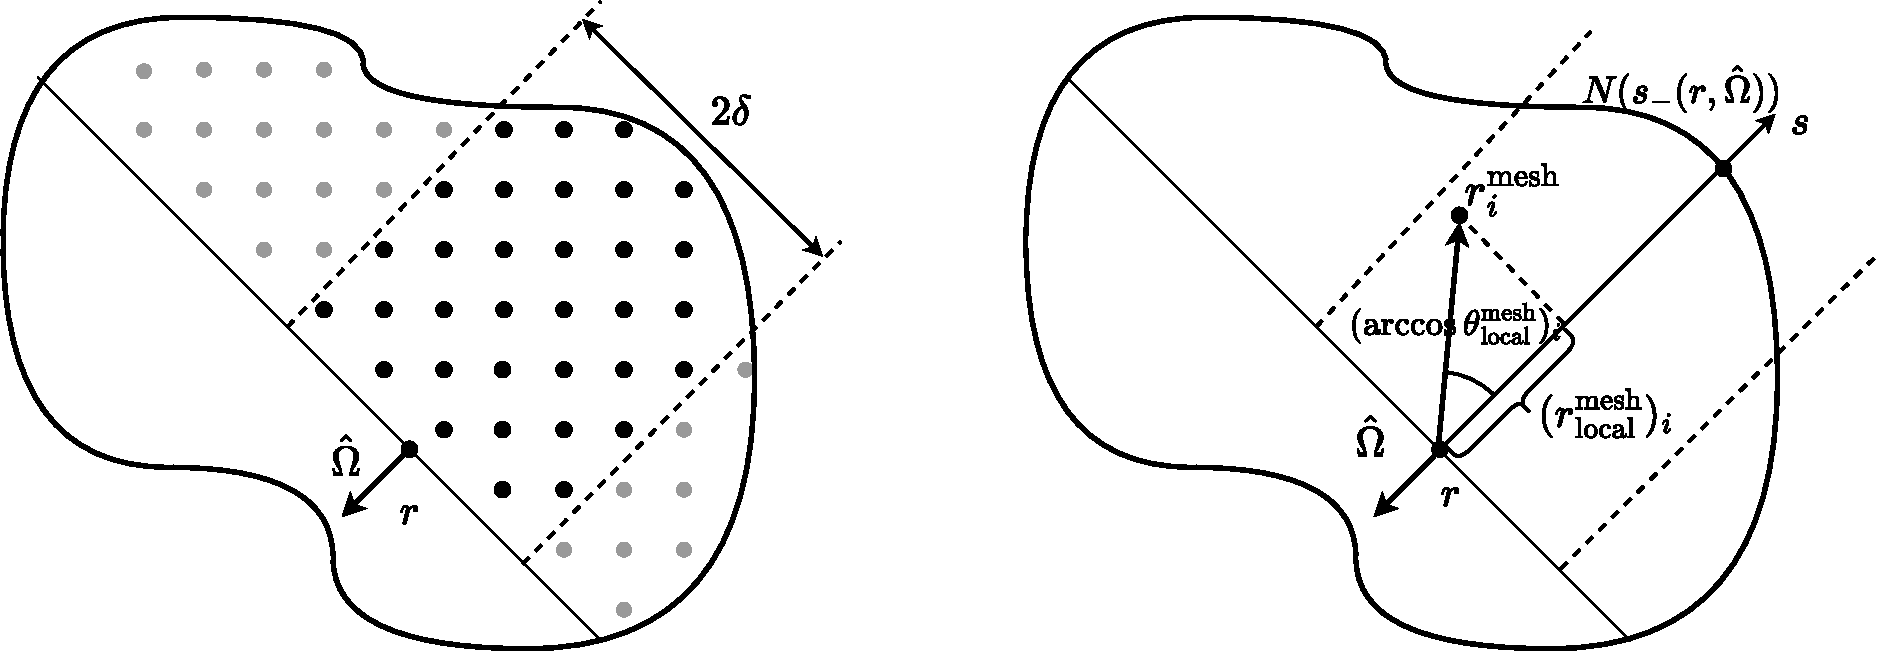
\includegraphics[width=.8\textwidth]{figures/mask.pdf}
    \bicaption{掩码和相对位置嵌入。实心点表示特征线 $\delta$-邻域内的活动网格节点。这些节点为光学深度插值提供空间支持，从而避免全域计算。}{Mask and relative position embedding. Solid dots represent active grid nodes within the $\delta$-neighborhood of the characteristic line. These nodes provide spatial support for optical depth interpolation, thereby avoiding full-domain computation.}\label{fig:mask}
\end{figure}
\begin{equation}
    \mathcal{C}_{\br,\bOmega} = \left \{\rmesh_i \mid \text{distance}\left(\rmesh_i, \{\br - s\bOmega, s\in(0,s_-(\br,\bOmega))\}\right) < \delta\right \}.
\end{equation}
这表明，只有靠近特征线的网格点才会对光学深度计算产生非零贡献。

更具体地说，$\br^{\text{mesh}}_i$ 与第 $j$ 个求积点 $\br-s_j \bOmega$ 的相对位置，可通过其在特征线方向上的投影以及向量 $\br^{\text{mesh}}_i-\br$ 与特征线之间的夹角来刻画（见图~\ref{fig:mask}）。
注意到 $\|\bOmega \| = 1$ 且特征线位于 $\bOmega$ 的相反方向，我们有
\begin{equation}
    \begin{cases}
        {(r^\text{mesh}_\text{local})}_i      & = -(\br^\text{mesh}_i - \br)\cdot \bOmega,                          \\
        {(\theta^\text{mesh}_\text{local})}_i & = {(r^\text{mesh}_\text{local})}_i / \| \br^\text{mesh}_i - \br \|,
    \end{cases}
\end{equation}
参见算法~\ref{alg:relative-position-encoding}，然后
\begin{equation}
    c(\br-s_j\bOmega, \br^{\text{mesh}}_i) = c\left(s_j; {(r^\text{mesh}_\text{local})}_i, {(\theta^\text{mesh}_\text{local})}_i\right).
\end{equation}
\begin{algorithm}[htp!]
    \caption{相对位置编码（Relative Position Encoding）}\label{alg:relative-position-encoding}
    \SetAlgoLined
    \KwIn{$\br, \bOmega, \tilde{\br}$}
    \KwOut{$(r_\text{local},\theta_\text{local}), m$}

    \emph{计算相对位置向量}\;
    $\br_{\text{rel}} = \br - \tilde{\br}$\;

    \emph{计算局部坐标系下的分量}\;
    $r_{\text{local}} =  \br_{\text{rel}} \cdot \bOmega$\;
    $\theta_{\text{local}} = r_{\text{local}}/\|\br_{\text{local}}\|$\;

    \emph{生成沿特征线的掩码}\;
    $m = -10^{10} \text{ if } s_\text{local} < 0 \text{ else } 0$\;

    \Return{$(r_\text{local},\theta_\text{local}), m$}\;
\end{algorithm}
基于上述观察，可以将光学深度近似为
\begin{equation}
    \begin{aligned}
        \tau_{-,t}(\br,\bOmega) & \approx \sum_j^{N\left(s_{-}(\br,\bOmega)\right)} w(\br, \bOmega;s_j)\sum_{i}^{N_\text{mesh}} \bm{1}_\mathcal{C}(\rmesh_i)c\left(s_j; {(r^\text{mesh}_\text{local})}_i, {(\theta^\text{mesh}_\text{local})}_i\right){(\mu_t^\text{mesh})}_i         \\
                                & =\sum_{i}^{N_\text{mesh}} \bm{1}_\mathcal{C}(\rmesh_i)\left(\sum_{j}^{N\left(s_{-}(\br,\bOmega)\right)} w(\br, \bOmega;s_j)c\left(s_j; {(r^\text{mesh}_\text{local})}_i, {(\theta^\text{mesh}_\text{local})}_i\right)\right){(\mu_t^\text{mesh})}_i \\
                                & =\sum_{i}^{N_\text{mesh}} \underbrace{\bm{1}_\mathcal{C}(\rmesh_i)W(\br,\bOmega; {(r^\text{mesh}_\text{local})}_i, {(\theta^\text{mesh}_\text{local})}_i)}_{\text{attention weights}}\underbrace{{(\mu_t^\text{mesh})}_i}_{\text{values}},
        % & \approx \sum_{i}^{N_\text{mesh}} \left(\sum_{m}^{d_k} w_m(\br,\bOmega)w_m\left((r_\text{local})_i, (\theta_\text{local})_i\right)\right)\mut(\br_i^{\text{mesh}}).
    \end{aligned}
\end{equation}
这里，我们首先对 $j$ 作内部求和，以确定系数 $W\left(\br,\bOmega; {(r_\text{local})}_i, {(\theta_\text{local})}_i\right)$，可理解为每个网格点对光学深度积分的综合贡献。

在连续层面上，该权重与 $N\left(s_{-}(\br,\bOmega)\right)$ 及具体采样点 $s_j$ 的选择无关；在离散实现中也可保持类似性质。这一点十分关键，因为求积点本身并未在网络结构中显式出现。系数 $W$ 实际上承担了相空间点 $(\br,\bOmega)$ 与网格点 $\br_i^{\text{mesh}}$（通过其局部坐标表示）之间相关性的角色。
从另一个角度看，系数 $W$ 可由多头注意力机制学习，其中查询为相空间点 $(\br,\bOmega)$，键为网格点的局部坐标，值则为总截面取值 $\mu_t(\br_i^{\text{mesh}})$，对应的近似为
\begin{equation}
    W\left(\br,\bOmega; {\left(r^\text{mesh}_\text{local}\right)}_i, {\left(\theta^\text{mesh}_\text{local}\right)}_i\right) \approx \sum_{m}^{d_k} \underbrace{q_m(\br,\bOmega)}_{\text{query}:\;QW^Q_h}\underbrace{k_m({(r^\text{mesh}_\text{local})}_i, {(\theta^\text{mesh}_\text{local})}_i)}_{\text{keys}:\;KW^K_h},
    % & \approx \text{softmax}\left((QW_h^Q) (KW_h^K)^T / \sqrt{d_k} + M\right),
\end{equation}
其中 $d_k$ 为键空间维度的超参数，$w_m$ 表示多头注意力中的第 $m$ 个通道。
指示函数 $\bm{1}_\mathcal{C}(\rmesh_i)$ 则通过掩码 $M$ 与 softmax 函数联合实现：
\begin{equation}
    \text{softmax}_i(\bm{x}) = \frac{e^{x_i+m_i}}{\sum_j e^{x_j+m_j}},
\end{equation}
其中，当网格点 $\rmesh_i$ 不属于集合 $\mathcal{C}$ 时取 $m_i=-10^{10}$，否则取 $0$，从而保证远离特征线的网格点对应的注意力权重近似为零。

实现中，我们用法向量为速度反方向的半平面生成掩码 $M$，从而屏蔽远离特征线的网格点（见图~\ref{fig:mask}）。掩码的宽度可按需求调节：更宽的范围捕捉更复杂的光学深度变化，更窄的范围则进一步提升计算速度。

综合上述要素，可得到算法~\ref{alg:optical-depth-net} 所示的 OpticalDepthNet 计算流程：

\begin{algorithm}[htp!]
    \caption{光学深度网络（Optical Depth Network）}\label{alg:optical-depth-net}
    \SetAlgoLined
    \KwIn{$\br, \bOmega, \{\br_i^{\text{mesh}}\}, \{{(\mut^{\text{mesh}})}_i\}, \{{(\mus^{\text{mesh}})}_i\}, d_k=12, H=2$}
    \KwOut{$\tau_{-}$}

    \emph{计算网格点的相对位置编码}\;
    ${(\br^\text{mesh}_{\text{local}})}_i, m_i = \hyperref[alg:relative-position-encoding]{\text{RelativePositionEncoding}}(\br, \bOmega, \br_i^{\text{mesh}})$\;

    \emph{将输入投影到多头注意力空间, $\bm{q}^h, \bm{k}_i^h \in \mathbb{R}^{d_k}, \bm{v}_i^h \in \mathbb{R}^{d_v}$}\;
    $\bm{q}^h = \text{LinearNoBias}((\br,\bOmega))$\;
    $\bm{k}_i^h = \text{LinearNoBias}\left({(\br^\text{mesh}_{\text{local}})}_i\right)$\;
    $\bm{v}_i^h = \text{LinearNoBias}\left(\text{concat}\left({(\mut^{\text{mesh}})}_i,{(\mus^{\text{mesh}})}_i\right)\right)$\;

    \emph{计算注意力权重并聚合值, $\bm{\tau}^h\in\R^{d_v}$}\;
    $a_{i}^h = \text{softmax}_i\left(\frac{1}{\sqrt{d_k}}{(\bm{q}^h)}^{\transpose}\bm{k}_i^h+m_i\right)$\;
    $\bm{\tau}^h = \sum_i a_{i}^h \bm{v}_i^h$\;

    \emph{拼接多头输出并投影, $\tau_{-}\in \mathbb{R}^{d_\tau}$}\;
    $\tau_{-} = \text{LinearNoBias}\left(\text{concat}_h(\bm{\tau}^h)\right)$\;

    \Return{$\tau_{-}$}\;
\end{algorithm}


\subsection{散射模块}\label{sec:scattering-module}
散射模块用于刻画多次散射效应，其设计基于~\eqref{eq:greens-function-series} 中算子 $G$ 的级数展开。对应的网络结构如图~\ref{fig:scattering-module} 所示，可写作
\begin{equation}
    \begin{aligned}
         & \bG^{0} = \bG^{\text{NN}}(\br,\bOmega,\br^{\prime},\bOmega^{\prime}),                               \\
         & \bG^{\ell}  = \text{ScatteringBlock}_{\ell}(\bG^{\ell-1}) + \bG^{0}, \quad \ell = 1,\dots,N_{\ell},
    \end{aligned}
\end{equation}
其中 $\text{ScatteringBlock}_\ell$（如图~\ref{fig:scattering-block}所示）定义为
\begin{equation}\label{eq:scattering-block}
    \text{ScatteringBlock}_\ell(\bm{G}) = \text{LayerNorm}\Big(\sigma\Big(\bm{W}^{\ell} \bm{S}^{\top} \bm{G} + \bm{b}^{\ell}\Big)\Big).
\end{equation}

与不动点迭代式~\eqref{eq:fixed-point-iteration} 对比可知，散射块可视为对算子 $\cL\cS$ 的一次近似作用。这里 $\bm{W}^{\ell} \in \mathbb{R}^{d_{\text{model}}\times d_{\text{model}}}$ 和 $\bm{b}^{\ell} \in \mathbb{R}^{d_{\text{model}}}$ 为可学习的线性变换参数，而 $\bm{S} = \big[\, w_i\, p(\bOmega, \bOmega_i^*) \,\big]_{j=1}^{d_{\text{quad}}}$ 则给出~\eqref{eq:scattering-op} 中散射算子的数值求积近似。$\sigma(x)$ 表示激活函数，在本文中取 $\tanh(x)$。

归一化层遵循文献，具有可训练的仿射参数 $\bm{\gamma},\bm{\beta} \in \mathbb{R}^{d_{\text{model}}}$
\begin{equation}
    \text{LayerNorm}(\bm{x}) = \frac{\bm{x}-\alpha\bm{1}}{\sigma}\cdot\bm{\gamma} + \bm{\beta}, \quad\alpha=\sum_{i=1}^{d_{\text{model}}}\frac{x_i}{d_\text{model}}, \quad\sigma=\sqrt{\sum_{i=1}^{d_{\text{model}}}\frac{{(x_i-\alpha)}^2}{d_\text{model}}}.
\end{equation}
层归一化有助于提升~\eqref{eq:greens-function-iterations} 所描述递归过程的数值稳定性。如果权重矩阵 $\bm{W}^\ell$ 病态或接近奇异，反复迭代会放大误差并削弱收敛性质；层归一化则在一定程度上抑制了这类问题，使训练更稳定高效。实践中常见的两种用法为：
\begin{itemize}
    \item \textbf{Post-Norm}：归一化应用于散射算子之后。这种直接的方法在浅层网络中表现良好。
    \item \textbf{Pre-Norm}：归一化应用于散射算子之前。这种方法可以缓解深层网络中的梯度问题。
\end{itemize}
在对比两种实现方式后，我们在散射块中采用后归一化（Post-Layer Normalization）结构，以在训练稳定性与实现简洁性之间取得平衡。

\begin{figure}[htp!]
    \centering
    
\includegraphics[width=0.9\textwidth]{scattering_module.pdf}
    \bicaption{散射模块。}{Scattering module.}\label{fig:scattering-module}
\end{figure}


图~\ref{fig:scattering-module}展示了散射模块的基本思路，即堆叠残差块，结合物理先验的 $\cS$ 近似层，并采用 tanh 激活的算子变换与自适应层归一化以稳定训练。

\begin{figure}[htp!]
    \centering
    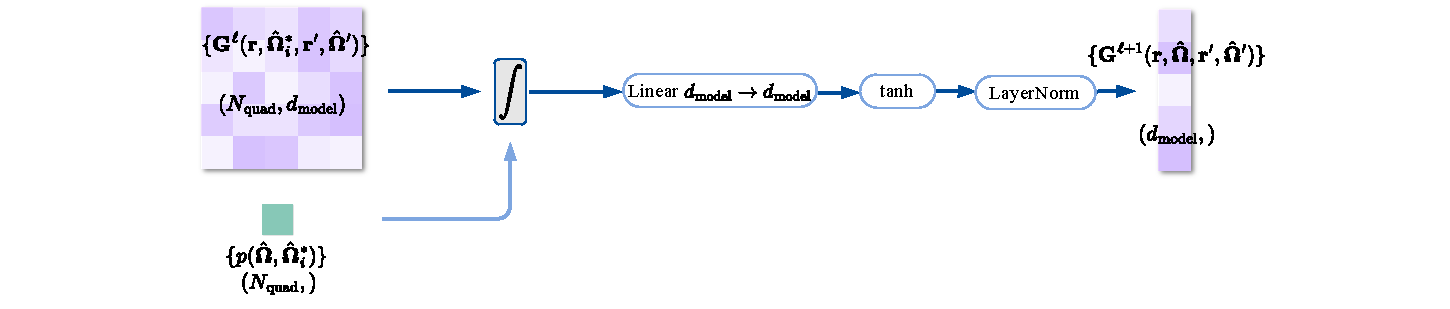
\includegraphics[width=1\textwidth]{figures/scattering_block.pdf}
    \bicaption{散射块。}{Scattering block.}\label{fig:scattering-block}
\end{figure}

图~\ref{fig:scattering-block}表示模拟算子 $\cS$ 作用一次的结果。包括积分的加权求和、线性投影和激活。

\noindent 散射模块的详细算法在算法~\ref{alg:scattering-module}中提供。

\begin{algorithm}[htp!]
    \caption{散射模块（Scattering Module）}\label{alg:scattering-module}
    \SetAlgoLined
    \KwIn{$\bm{g}, \{\bm{g}^*_j\}, \{p(\bOmega,\bOmega^*_i)\},\{p(\bOmega^*_i,\bOmega^*_j)\}, \{w_j\}, N_s=2$}
    \KwOut{$\bm{g}$}

    \emph{保存初始状态用于残差连接, ${(\bm{g}^*_j)}^{\text{init}}\in \mathbb{R}^{d_{\text{model}}}$}\;
    ${(\bm{g}^*_j)}^{\text{init}} = \bm{g}^*_j$\;

    \emph{执行带有跳跃连接的散射块迭代}\;
    \For{$\ell\in[0,\ldots,N_\ell-2]$}{
    \emph{添加初始值以模拟级数展开, $\bm{g}^*_i\in \mathbb{R}^{d_{\text{model}}}$}\;
    $\bm{g}^*_i\gets{(\bm{g}^*_i)}^{\text{init}} + \hyperref[alg:scattering-block]{\text{ScatteringBlock}_\ell}(\{\bm{g}^*_j\},\{p(\bOmega^*_i,\bOmega^*_j), \{w_j\} \}) $\;
        }

    $\bm{g}\mathrel{+}=\hyperref[alg:scattering-block]{\text{ScatteringBlock}_{N_\ell-1}}(\{\bm{g}^*_i\},\{p(\bOmega,\bOmega^*_i)\}, \{\omega_i\})$ \hfill \emph{$\bm{g}\in \mathbb{R}^{d_{\text{model}}}$} \;

    \Return{$\bm{g}$}\;
\end{algorithm}

\subsubsection{散射块}
基于~\eqref{eq:soln-op-series} 的级数展开，我们定义沿特征线的截断状态向量，用以刻画离散采样点处的辐射场：

\begin{equation}
    \bG^{\ell} =
    \begin{pmatrix}
        G^\ell(\br-s_1 \bOmega, \bOmega; \br', \bOmega') \\
        \vdots                                           \\
        G^\ell(\br-s_{d_{\text{model}}} \bOmega, \bOmega; \br', \bOmega')
    \end{pmatrix}\in \mathbb{R}^{d_{\text{model}}},
\end{equation}
其中 $\bG^0$ 由衰减模块提供的初始格林函数表示。由此可得到如下递推关系：
\begin{equation}
    G^{\ell+1} = \cL\cS G^\ell + G^0.
\end{equation}
算子 $\cL\cS$ 由两个物理过程组成：(1) 角度散射 $\cS$；(2) 沿特征线的提升 $\cL$。其积分表示为
\begin{equation}\label{LS}
    \cL\cS G^{\ell}(\br, \bOmega) = \int_0^{s_{-}(\br, \bOmega)} e^{-\tau(0,s')}
    \mus(\br-s' \bOmega) \underbrace{\frac{1}{S_d} \int_{\sS^{d-1}}
        p(\bOmega, \bOmega^*) G^{\ell}(\br-s' \bOmega, \bOmega^*)
        \diff{\bOmega^*}}_{\cS G^{\ell}(\br-s' \bOmega, \bOmega)} \diff{s'}.
\end{equation}

\paragraph{数值实现}
为保持计算的可行性，我们首先使用角度求积近似散射算子 $\cS$：

\begin{equation}
    \cS G^\ell(\br-s' \bOmega, \bOmega) \approx \sum_{i=1}^{d_{\text{quad}}} w_i p(\bOmega, \bOmega_i^*) G^{\ell}(\br-s' \bOmega, \bOmega_i^*),
\end{equation}
其中 $d_{\text{quad}}$ 个带有权重 $\{w_i\}$ 的求积点近似角度积分。

进一步地，为近似 \eqref{LS} 右侧沿特征线的积分，我们引入离散散射近似：
\begin{equation}
    \cL\cS G^{\ell}(\br, \bOmega) \approx \sum_{j=1}^{d_{\text{model}}} \tilde{w}_j^{\br, \Omega} \mus e^{-\tau(0,s'_j)} \cS G^\ell(\br-s'_j \bOmega, \bOmega).
\end{equation}

为避免在训练过程中重复进行高成本的特征线积分计算，我们将传输算子整体参数化为可学习的权重矩阵：
\begin{equation}\label{eq:scattering-mus}
    \begin{aligned}
        \cL\cS G^{\ell}(\br-s'_i\bOmega, \bOmega) & \approx  \sum_{j=1}^{d_{\text{model}}} \underbrace{\tilde{w}_j^{\br-s'_i \bOmega, \bOmega} \mus e^{-\tau(0,s'_j)}}_{w^\cL_{ij}} \cS{G}^{\ell}(\br-s'_j \bOmega, \bOmega) \\
                                                  & = \bm{w}^\cL_{i} {\cS \bG}^{\ell},
    \end{aligned}
\end{equation}
% \begin{equation}
%   \begin{aligned}
%     \cL\cS G^{\ell}(\br-s'_i\bOmega, \bOmega) & \approx \sum_{j=1}^{d_{\text{model}}} \tilde{w}_j^{\br-s'_i \bOmega, \bOmega} \mus e^{-\tau(0,s'_j)} \cS{G}^{\ell}(\br-s'_j \bOmega, \bOmega)\\
%     & = \bm{w}^\cL_{i} {\cS \bG}^{\ell},
%   \end{aligned}
% \end{equation}
其中 $\bm{w}^\cL_{i} = (w^\cL_{i1}, w^\cL_{i2}, \cdots, w^\cL_{id_{\text{model}}}) \in \mathbb{R}^{d_{\text{model}}}$。
完整的系统表示为：

\begin{equation}
    \bG^{\ell} =
    \begin{pmatrix}
        G^{\ell}(\br-s_1 \bOmega, \bOmega) \\
        \vdots                             \\
        G^{\ell}(\br-s_{d_{\text{model}}} \bOmega, \bOmega)
    \end{pmatrix}, \quad
    \mathbf{W}^\ell =
    \begin{pmatrix}
        \bm{w}^\cL_1 \\
        \vdots       \\
        \bm{w}^\cL_{d_{\text{model}}}
    \end{pmatrix}.
\end{equation}

\paragraph{神经网络实现}
在实际实现中，将 $\bm{W}^\ell$ 视为完全可学习的参数矩阵，由网络自动从数据中学习不同特征线采样点之间的最优耦合关系。此时散射块可简化为

\begin{equation}\label{scattering_layer}
    \text{ScatteringBlock}_\ell(\bm{G}) = \text{LayerNorm}\Big(\sigma\Big(\bm{W}^{\ell} \bm{S}^{\top} \bm{G} + \bm{b}^{\ell}\Big)\Big),
\end{equation}
其中 $\bm{W}^{\ell} \in \mathbb{R}^{d_{\text{model}}\times d_{\text{model}}}$ 以数据驱动的方式编码了传输物理和数值求积权重。

散射块的详细计算步骤在算法~\ref{alg:scattering-block} 中给出。

\begin{algorithm}[htp!]
    \caption{散射块（Scattering Block）}\label{alg:scattering-block}
    \SetAlgoLined
    \KwIn{$\{\bm{g}_i\}, \{p_i\}, \{\omega_i\}, d_{\text{model}}=16$}
    \KwOut{$\bm{g}$}

    \emph{通过加权求和近似数值积分}\;
    $\bm{g}  = \sum_i \omega_i p_i \bm{g}_i$\;

    \emph{应用线性变换和激活函数, $\bm{g}\in \mathbb{R}^{d_{\text{model}}}$}\;
    $\bm{g}\gets \text{tanh}\left(\text{Linear}( \bm{g})\right)$\;

    \emph{应用层归一化}\;
    $\bm{g} \gets \text{LayerNorm}(\bm{g})$\;

    \Return{$\bm{g}$}\;
\end{algorithm}


为了将 $\mus e^{-\tau(0,s'_j)}$ 编码到散射模块中，我们在方程~\eqref{eq:scattering-block}中构造权重 $\bm{W}^\ell$ 如下：
\begin{equation}
    \mathbf{W}^\ell =
    \begin{pmatrix}
        \bm{w}^\cL_1 \\
        \vdots       \\
        \bm{w}^\cL_{d_{\text{model}}}
    \end{pmatrix}
    =
    \begin{pmatrix}
        \tilde{w}_j^{\br-s'_1 \bOmega, \bOmega}\circ \tau^{NN}_{-,s} \\
        \vdots                                                       \\
        \tilde{w}_j^{\br-s'_{d_\mathrm{model}} \bOmega, \bOmega} \circ \tau^{NN}_{-,s}
    \end{pmatrix},
\end{equation}
其中 $\tau^{NN}_{-,s} \approx ( \mus(\br-s'_1\bOmega) e^{-\tau(0,s'_1)}, \mus(\br-s'_2\bOmega) e^{-\tau(0,s'_2)}, \cdots, \mus(\br-s'_{d_{\mathrm{model}}}\bOmega) e^{-\tau(0,s'_{d_{\mathrm{model}}})} )$。我们观察到 $\tau(0,s'_j)$ 可以使用类似于我们衰减模块的基于注意力的架构来建模。完整的计算序列——评估 $\tau(0,s'_j)$、应用指数以及乘以 $\mus$——由神经网络端到端地近似。

在具体实现中，该网络与 $\tau^{NN}_{-,t}$ 一并集成在衰减模块中，$\mathrm{OpticalDepthNet}$ 的输出为拼接后的向量 $\tau_- = \mathrm{Concat}(\tau^{NN}_{-,t}, \tau^{NN}_{-,s})$。这一设计在算法~\ref{alg:optical-depth-net} 中被形式化，其中
\begin{equation}
    \tau_- = \mathrm{Concat}\left(\tau^{NN}_{-,t}, \tau^{NN}_{-,s}\right) = \mathrm{OpticalDepthNet}\left(\br,\bOmega; \{\br^{\mathrm{mesh}}_i\}, \left\{(\mu_t^{\mathrm{mesh}}, \mu_s^{\mathrm{mesh}})_i\right\}\right) \in \mathbb{R}^{d_{\tau}},
\end{equation}
其中 $d_\tau > d_{\mathrm{model}}$。

\subsection{模块优势与特点}

衰减模块的设计赋予了 DeepRTE 显著的灵活性和计算优势，主要体现在以下几个方面：

\begin{itemize}
    \item \textbf{网格选取的自由性}：这是本模块最核心的优势。输入网格点 $\{\br^{\text{mesh}}_i\}$ 仅用于刻画介质参数 $\mu_t$ 和 $\mu_s$ 的空间分布，而与辐射场 $I$ 的求解位置完全解耦。这意味着：
          \begin{enumerate}
              \item 网格点不必与求解点重合，也不受求解区域几何形状的限制。
              \item 对于 $\mu_t$ 变化平缓或分段常数的区域，可以使用非常稀疏的网格来精确表示介质属性，从而大幅降低计算量。
              \item 支持非结构化网格，能够灵活适应复杂的介质分布。
          \end{enumerate}

    \item \textbf{计算效率与精度的平衡}：在实际应用中，虽然默认使用全场网格点参与计算以保证通用性，但该架构天然支持局部化策略。在大规模三维问题中，可以仅选取特征线邻域内的网格点子集参与注意力计算（如带状区域等），从而在保持精度的同时显著提升推理速度。
\end{itemize}

在散射模块中，\eqref{eq:scattering-mus}引入了可学习的权重 $\bm{w}^\cL_{ij} = \tilde{w}_j^{\br-s'_i \bOmega, \bOmega} \mus e^{-\tau(0,s'_j)}$，这会带来一个疑问，即训练结束的权重是一个固定的值，但是$\bm{w}^\cL_{ij}$中出现的 $\mus$ 和 $\tau$ 实际上是输入相关的变量，虽然我们将$\mut$，$\mus$拼接在一起作为OpticalDepthNet的输入并传入散射模块以补足$\mus$的信息，但是这种与物理形式有差异的设计否会导致表达能力受限？

为此，我们对比了两套网络设计。
首先，我们把符合物理意义的 $\bm{w}^\cL_{ij}$ 进行了实验的复现。具体来说，我们使用与衰减模块中相同的 OpticalDepthNet 来预测 $\tau(0,s'_j)$，并将 $\mus$ 从输入中直接提取出来计算 $\bm{w}^\cL_{ij}$。然后，将原衰减模块的输出$\bm{G}^{\text{NN}}$ 与 $\bm{w}^\cL_{ij}$ 拼接，形成散射模块的输入，即:
\begin{equation}
    \begin{aligned}
        \bm{G}^{0}         & = \mathrm{Concat}\left(\bm{G}^{\text{NN}}, \mathbf{W}^\ell\right),             \\
        \bm{G}^{\text{NN}} & =
        \begin{pmatrix}
            G^{\text{NN}}(\br-s_1 \bOmega, \bOmega; \br', \bOmega') \\
            \vdots                                                  \\
            G^{\text{NN}}(\br-s_{d_{\text{model}}} \bOmega, \bOmega; \br', \bOmega')
        \end{pmatrix}, \\
        \mathbf{W}^\ell    & =
        \begin{pmatrix}
            \bm{w}^\cL_1 \\
            \vdots       \\
            \bm{w}^\cL_{d_{\text{model}}}
        \end{pmatrix},
    \end{aligned}
\end{equation}
其中 $\bm{w}^\cL_{ij} = \tilde{w}_j^{\br-s'_i \bOmega, \bOmega} \mus(\br-s'_j\bOmega) e^{-\tau^{NN}_{-,s}(0,s'_j)}$。

最后将上述的 $\bm{G}^0$ 输入到~\eqref{scattering_layer}中进行散射模块的实现，最后的迭代网络结构与之前保持一致。上述实现更改了散射模块的输入形式，但并未改变散射块的结构，使得网络满足了物理意义上的 $\bm{w}^\cL_{ij}$ 形式。

第二种实现则是我们在前文中介绍的直接学习 $\bm{W}^\ell$ 的方式。将$\mut$，$\mus$拼接在一起作为OpticalDepthNet的输入，详情见算法~\ref{alg:optical-depth-net}。

实验结果表明，这两种方式的表现相差无几。这说明，我们将$\mut$，$\mus$作为衰减输入的设计是合理且有效的。
